%\documentclass[11pt]{article}
%\usepackage{graphicx}
%\usepackage{amssymb}
%\usepackage{epstopdf}
%\usepackage{doublespace}
%\DeclareGraphicsRule{.tif}{png}{.png}{`convert #1 `dirname #1`/`basename #1 .tif`.png}

%\textwidth = 6.5 in
%\textheight = 9 in
%\oddsidemargin = 0.0 in
%\evensidemargin = 0.0 in
%\topmargin = 0.0 in
%\headheight = 0.0 in
%\headsep = 0.0 in
%\parskip = 0.2in
%\parindent = 0.0in

%\newtheorem{theorem}{Theorem}
%\newtheorem{corollary}[theorem]{Corollary}
%\newtheorem{definition}{Definition}

%\title{Matrix Multiply Results}
%\author{Daniel D. Beatty}
%\begin{document}
%\maketitle

%\chapter


Each empirical result is from % either 
a series of matrix multiplications on 9 different images.  These matrices were submitted to preconditioning with the wavelet transform in the 3 basic method of decomposition --- MRA, MRE and the $\psi^n$ decomposition.%   with wavelet packets or wavelet pyramids type wavelet transforms.  
In the end, MRA performed poorly for any set of resolutions deeper than one in matrix multiplication.  Thus MRA should not be used as a pre-conditioner to matrix multiplication.  The MRE transform performs modestly in matrix multiplication tests, but to be effective must be reordered into $\psi^n$ structure. %require reordering to match the recursive MRE wavelet transform packet form.    
Lastly, the $\psi^n$ form performs well on matrix multiplication.   

The matrix multiplication used in each of these cases is %a special case of matrix multiplication is conducted, 
$A^2= A\cdot A$, where $A$ is  a $M\times N$ matrix.  The general equation for evaluating the wavelet transform pyramid method is the fidelity measurement:
\[
\sqrt{E(\psi^{-1} ( (\psi (A))^2) - A^2)}.
\]
where $\psi$ represents the given multilevel wavelet transform and $\psi^{-1}$ represents its inverse. Relative fidelity measurements provide an error that takes into account the scale. It is more useful for general observations.  To obtain this measurement, the results are compared to standard.  % reference of a standard.  
In this case, $A^2$ is the standard, and the energy difference is inversely proportional.
\[ \sqrt {\frac{E(\psi^{-1} ( (\psi (A))^2) - A^2)} {E(A^2)} }  \]
In both fidelity and relative fidelity, the energy of the function is defined.  
\[
E(A) = \frac{1}{m\cdot n} \sum\limits_{i=0}^{m-1} \sum\limits_{j=0}^{n-1} (a_{i,j})^2
\]

%\section {Matrix Multiplication Results}
%\{tiny}



\section{$8\times 8$ Examples}
This section demonstrates matrix multiplication on $\psi^n$ expanded $8\times8$ matrix multiplication.  % a test simple $8\times 8$ matrices multiplied in wavelet space.  
One matrix in the set is an upper triangular matrix it is multiplied by itself.  %and multiplies it by itself.  
Another is a matrix of $\frac{1}{2}$s everywhere except the diagonal being $\frac{1}{4}$ and it is also multiplied by itself.  In the third example, the  upper triangular matrix and matrix of $\frac{1}{2}$ are multiplied together.  

The values are inserted and retrieved from the program in PGM and PPM formats with their signs retained.  Also, values above 256 and below zero are retained.  Each value is a quantized by 256 during the input and output stages.  While processing, the values are computed with double floating point precision.  In these case, the only error can be accounted for by quantization and numerical round off at the output.

\subsection{Matrix multiplication on $8\times 8$ Upper Triangle} \label{sec:uppertriangle}
This first example of multiplication uses the matrix defined in equation \ref{equ:basea} as the test matrix $A$.   $A^2$ is provided in equation \ref{equ:basea2}.  %, the results of matrix multiply of $A^2$ is presented.  $A$ is simple, and its results in fractional and decimal form are provided.  In the sub-sections that follow the one, two and three resolution wavelet transform and the multiplications for $A^2$ are provided.  In each section, the conventional $A^2$ is referenced for comparison.   
%In the following sub-sections, Matrix multiply is performed on the CWT of $A$  for the following expansions: $\psi^1$, $\psi^2$, and $\psi^3$.  In each case, the inverse transform is applied to the product, and that inverse is compared with equation \ref{equ:basea2}.  

\begin{equation}
\label{equ:basea}A= \frac{1}{256} \left(
\begin{array}{cccccccc}
64 & 128 & 128 & 128 & 128 & 128 & 128 & 128 \\ 
0 & 64 & 128 & 128 & 128 & 128 & 128 & 128 \\ 
0 & 0 & 64 & 128 & 128 & 128 & 128 & 128 \\ 
0 & 0 & 0 & 64 & 128 & 128 & 128 & 128 \\ 
0 & 0 & 0 & 0 & 64 & 128 & 128 & 128 \\ 
0 & 0 & 0 & 0 & 0 & 64 & 128 & 128 \\ 
0 & 0 & 0 & 0 & 0 & 0 & 64 & 128 \\ 
0 & 0 & 0 & 0 & 0 & 0 & 0 & 64
\end{array}\right)
\end{equation}
\begin{equation}
\label{equ:basea2}
A^2
=\allowbreak \frac{1}{256}\left(
\begin{array}{cccccccc}
17 & 65 & 129 & 193 & 258 & 322 & 386 & 450\\
0 & 17 & 65 & 129 & 193 & 258 & 322 & 386\\
0 & 0 & 17 & 65 & 129 & 193 & 258 & 322\\ 
0 & 0 & 0 & 17 & 65 & 129 & 193 & 258\\ 
0 & 0 & 0 & 0 & 17 & 65 & 129 & 193\\
0 & 0 & 0 & 0 & 0 & 17 & 65 & 129\\
0 & 0 & 0 & 0 & 0 & 0 & 17 & 65\\
0 & 0 & 0 & 0 & 0 & 0 & 0 & 17 
\end{array} \right)
\end{equation}

The steps and notation for analyzing the $\psi^3$ expansion of $A$ are listed here:
\begin{itemize}
\item $W^3(A)$ is the $\psi^3$ expansion of $A$ and is shown in equation \ref{equ:w3aexamp}.
\item $(W^3(A))^2$ is the square of $W^3(A)$ and is shown in equation \ref{equ:w3aexamp}.
\item $W^{-3}((W^3(A))^2)$ is the $\psi^-3$ inverse of $(W^3(A))^2$. and is shown in equation \ref{equ: invw3aexamp2}.
\end{itemize}
The $\psi^3$ expansion of $A$ has six elements of the 64 elements are below $\frac{1}{512}$.  Another ten of the 64 elements are below $\frac{3}{512}$.    Relative fidelity is on the order of $10^-14$. 

\begin{equation}
\label{equ:w3aexamp}
W^3(A)= \frac{1}{256} \left(
\begin{array}{cccccccc}
512 & 64 & 128 & 0 & 256 & 0 & 0 & 0\\
-64 & 0 & 0 & 1 & 0 & 0 & 0 & 0\\
-128 & 0 & 0 & 65 & 0 & 1 & 1 & 1\\
1 & 1 & -64 & 0 & 1 & 1 & 0 & 0\\
-256 & 1 & 0 & 0 & 0 & 65 & 129 & 0\\
1 & 0 & 0 & 1 & -64 & 0 & 0 & 1\\
1 & 1 & 1 & 1 & -128 & 0 & 0 & 65\\
0 & 1 & 0 & 0 & 1 & 1 & -64 & 0 
\end{array} \right)
\end{equation}
\begin{equation}
\label{equ: w3aexamp2}
(W^3(A))^2= \frac{1}{256} \left(
\begin{array}{cccccccc}
691 & 129 & 258 & 33 & 515 & 65 & 129 & 0\\
-128 & -16 & -32 & 0 & -64 & 0 & 0 & 1\\
-257 & -32 & -80 & 1 & -128 & 0 & 0 & 1\\
33 & 1 & 1 & -16 & 1 & 0 & 0 & 0\\
-514 & -64 & -128 & 1 & -337 & 1 & 1 & 33\\
65 & 1 & 1 & 0 & 1 & -16 & -32 & 0\\
129 & 1 & 1 & 0 & 1 & -32 & -80 & 1\\
0 & 0 & 0 & 0 & 33 & 1 & 1 & -16 
\end{array} \right)
\end{equation}

\begin{equation}
\label{equ: invw3aexamp2}
W^-3((W^3(A))^2)= \frac{1}{256} \left(
\begin{array}{cccccccc}
17 & 65 & 129 & 193 & 258 & 322 & 386 & 450\\
0 & 17 & 65 & 129 & 193 & 258 & 322 & 386\\
0 & 0 & 17 & 65 & 129 & 193 & 258 & 322\\
0 & 0 & 0 & 17 & 65 & 129 & 193 & 258\\
0 & 0 & 0 & 0 & 17 & 65 & 129 & 193\\
0 & 0 & 0 & 0 & 0 & 17 & 65 & 129\\
0 & 0 & 0 & 0 & 0 & 0 & 17 & 65\\
0 & 0 & 0 & 0 & 0 & 0 & 0 & 17
\end{array} \right)
\end{equation}

\subsection{Matrix Multiply Results for 8 by 8 Full Matrix}\label{sec:fullmatrix}
This next example uses a matrix defined in equation \ref{equ:bexamp}, and designated $B$.  %This matrix is filled with nothing but $\frac{1}{2}$ except on the diagonal.  
The square of $B$ is denoted $B^2$ and is shown in equation \ref{equ:bexamp2}.  

\begin{equation}
\label{equ:bexamp}
B = \frac{1}{256} \left(
\begin{array}{cccccccc}
64 & 128 & 128 & 128 & 128 & 128 & 128 & 128 \\ 
128 & 64 & 128 & 128 & 128 & 128 & 128 & 128 \\ 
128 & 128 & 64 & 128 & 128 & 128 & 128 & 128 \\ 
128 & 128 & 128 & 64 & 128 & 128 & 128 & 128 \\ 
128 & 128 & 128 & 128 & 64 & 128 & 128 & 128 \\ 
128 & 128 & 128 & 128 & 128 & 64 & 128 & 128 \\ 
128 & 128 & 128 & 128 & 128 & 128 & 64 & 128 \\ 
128 & 128 & 128 & 128 & 128 & 128 & 128 & 64
\end{array} \right)
\end{equation}

\begin{equation}
\label{equ:bexamp2}
B^2 = \frac{1}{256}  \left(
\begin{array}{cccccccc}
466 & 450 & 450 & 450 & 450 & 450 & 450 & 450\\
450 & 466 & 450 & 450 & 450 & 450 & 450 & 450\\
450 & 450 & 466 & 450 & 450 & 450 & 450 & 450\\
450 & 450 & 450 & 466 & 450 & 450 & 450 & 450\\
450 & 450 & 450 & 450 & 466 & 450 & 450 & 450\\
450 & 450 & 450 & 450 & 450 & 466 & 450 & 450\\
450 & 450 & 450 & 450 & 450 & 450 & 466 & 450\\
450 & 450 & 450 & 450 & 450 & 450 & 450 & 466
\end{array} \right)
\end{equation}
The $\psi^3$ expansion of $B$ is denoted $W^3(B)$.  The procedure for computing $B^2$ in a $\psi^3$ expansion involves the follow:
\begin{itemize}
\item Compute the $\psi^3$ expansion denoted $(W^3(B))$ which is shown in equation \ref{equw3bexamp}.
\item Square $W^3(B)$, which is denoted $(W^3(B))^2$ and shown in equation \ref{equw3bexamp2}.
\item Compute the inverse of $(W^3(B))^2$, which is denoted as $W^{-3}((W^3(B))^2)$ and shown in equation \ref{equ:invw3bexamp2}.
\end{itemize}

\begin{equation}
\label {equw3bexamp}
W^3(B) = \frac{1}{256} \left(
\begin{array}{cccccccc}
961 & 0 & 0 & 0 & 0 & 1 & 1 & 1\\
0 & -64 & 0 & 1 & 0 & 1 & 1 & 0\\
0 & 1 & -63 & 1 & 0 & 1 & 1 & 0\\
1 & 1 & 1 & -64 & 0 & 0 & 1 & 1\\
1 & 1 & 1 & 1 & -63 & 1 & 1 & 1\\
1 & 1 & 0 & 0 & 1 & -64 & 1 & 1\\
0 & 1 & 1 & 0 & 1 & 1 & -63 & 1\\
0 & 0 & 1 & 1 & 0 & 1 & 1 & -64
\end{array} \right)
\end{equation}

\begin{equation}
\label {equw3bexamp2}
(W^3(B))^2 = \frac{1}{256} \left(
\begin{array}{cccccccc}
3615 & 0 & 0 & 0 & 0 & 0 & 1 & 1\\
0 & 17 & 1 & 0 & 1 & 0 & 0 & 1\\
0 & 1 & 17 & 0 & 1 & 0 & 0 & 1\\
0 & 0 & 0 & 17 & 0 & 1 & 1 & 0\\
1 & 0 & 0 & 0 & 17 & 0 & 0 & 1\\
1 & 0 & 0 & 1 & 0 & 17 & 1 & 0\\
1 & 1 & 0 & 1 & 0 & 1 & 17 & 0\\
0 & 1 & 1 & 0 & 1 & 0 & 0 & 17 
\end{array} \right)
\end{equation}

\begin{equation}
\label {equ:invw3bexamp2}
W^{-3}((W^3(B))^2) = \frac{1}{256} \left(
\begin{array}{cccccccc}
466 & 450 & 450 & 450 & 450 & 450 & 450 & 450\\
450 & 466 & 450 & 450 & 450 & 450 & 450 & 450\\
450 & 450 & 466 & 450 & 450 & 450 & 450 & 450\\
450 & 450 & 450 & 466 & 450 & 450 & 450 & 450\\
450 & 450 & 450 & 450 & 466 & 450 & 450 & 450\\
450 & 450 & 450 & 450 & 450 & 466 & 450 & 450\\
450 & 450 & 450 & 450 & 450 & 450 & 466 & 450\\
450 & 450 & 450 & 450 & 450 & 450 & 450 & 466
\end{array} \right)
\end{equation}

$W^3(B)$ has 14 of its elements with an epsilon of $\frac{1}{512}$.  Another, seven within an epsilon of $\frac{3}{512}$.  Most of the energy is in the second, third, fifth, and last rows.   The remaining energy is located in the diagonal.  Again nearly, $\frac{7}{32}$ of elements are not likely to contribute anything significant to this multiplication.   As for precision, the relative fidelity of  $W^{-3}((W^3(B))^2)$ and $B^2$ is on the order of $10^{-14}$.  


\subsection {Matrix Multiplication between Upper Triangular and Full Matrix}
This final $8\times 8$ example , the upper triangular matrix $A$ and a full matrix $B$ are multiplied together both in conventional space and in wavelet space.  Their results are compared for fidelity, and any notable discrepancies.  The upper triangular matrix is the same $A$ used in section \ref{sec:uppertriangle} .  The full matrix is the same $B$ used in section \ref{sec:fullmatrix}.  Their wavelet transforms are the same as in those sections as well.   The results of $(W^3(A) \cdot W^3(B))$ and $W^{-3}(W^3(A) \cdot W^3(B)))$ are described 
%Here the results for each resolution is described 
for completeness.  The product of $A$ and $B$ is designated $C$, and is % conventional matrix multiplication and is 
provided for comparison in equation \ref{equ:abexamp}.

\begin{equation}
\label {equ:abexamp}
A \cdot B = \frac{1}{256}\left( 
\begin{array}{cccccccc} 
466 & 450 & 450 & 450 & 450 & 450 & 450 & 450\\
418 & 402 & 386 & 386 & 386 & 386 & 386 & 386\\
354 & 354 & 338 & 322 & 322 & 322 & 322 & 322\\
290 & 290 & 290 & 274 & 258 & 258 & 258 & 258\\
225 & 225 & 225 & 225 & 209 & 193 & 193 & 193\\
161 & 161 & 161 & 161 & 161 & 145 & 129 & 129\\
97 & 97 & 97 & 97 & 97 & 97 & 81 & 65\\
33 & 33 & 33 & 33 & 33 & 33 & 33 & 17 
\end{array} \right)
\end{equation}

The multiplication of $A$ and $B$ in the $\psi^3$ expansion has a relative fidelity of  $2.3 \cdot 10^{-14}$.   The product of $A$ and $B$ in wavelet space is denoted $W^3(A) \cdot W^3(B)$, and its inverse is $W^{-3}(W^3(A) \cdot W^3(B))$.  
The matrix  $W(A)\cdot  W(B)$ is shown in equation \ref{equ:w3aw3bexamp}.  Its inverse, $W^{-3}(W^3(A) \cdot W^3(B))$, is shown in equation \ref{equ:invw3aw3bexamp}.
\begin{equation}
\label{equ:w3aw3bexamp}
W(A) \cdot W(B) = \frac{1}{256} \left(
\begin{array}{cccccccc}
1928 & -16 & -32 & 1 & -64 & 1 & 1 & 0\\
-240 & 1 & 1 & 0 & 1 & 0 & 0 & 0\\
-481 & 1 & 1 & -16 & 1 & 0 & 0 & 1\\
1 & 0 & 17 & 0 & 0 & 1 & 0 & 0\\
-963 & 1 & 1 & 0 & 1 & -16 & -32 & 1\\
1 & 0 & 0 & 0 & 17 & 0 & 1 & 0\\
1 & 0 & 0 & 1 & 33 & 0 & 1 & -16\\
0 & 1 & 0 & 0 & 0 & 0 & 17 & 0 
\end{array} \right)
\end{equation}
\begin{equation}
\label {equ:invw3aw3bexamp}
 W^{-1}(W(A) \cdot W(B)) = \frac{1}{256} \left(
\begin{array}{cccccccc}
466 & 450 & 450 & 450 & 450 & 450 & 450 & 450\\
418 & 402 & 386 & 386 & 386 & 386 & 386 & 386\\
354 & 354 & 338 & 322 & 322 & 322 & 322 & 322\\
290 & 290 & 290 & 274 & 258 & 258 & 258 & 258\\
225 & 225 & 225 & 225 & 209 & 193 & 193 & 193\\
161 & 161 & 161 & 161 & 161 & 145 & 129 & 129\\
97 & 97 & 97 & 97 & 97 & 97 & 81 & 65\\
33 & 33 & 33 & 33 & 33 & 33 & 33 & 17 
\end{array} \right)
\end{equation}


\section {Empirical Analysis: MRA}

Several standard images were used for measuring the effects of matrix multiplication.  Amongst them were the artificial images such as the waterfall and the clock.  Others were actual images such as an aerial view of the Pentagon, an in flight photo of an F-16, a fishing boat, an opera house, a river, and a set of bell peppers.

In first round analysis, matrix multiplication was measured against the wavelet pyramids.  These showed some undesirable results.  As the decomposition proceeded deeper, the fidelity quick became unstable, and made the method unusable for matrix multiplication.  The results are shown in Tables \ref{tbl:peppers_mra} and \ref{tbl:waterfall_mra}.

\begin{table}\caption{\label{tbl:peppers_mra}
Peppers $512 \times 512$ by MRA.}
\begin{center}
\begin{tabular}{clll}
{Resolution} & { Original Energy } & { 
Estimate Energy }& { 
Fidelity } \\ 
1&  12972.4& 12972.4 &  $1.26464 \cdot 10^{-13} $ \\ 
2&12972.4  & 12960.3 &  3.11211  \\ 
3& 12972.4 &12947.8  &  5.44678  \\ 
4&12972.4&12939.7&   8.43738 \\
5 &12972.4  & 12926 & 13.1662 \\
6& 12972.4& 12904.3& 19.9257 \\
7& 12972.4 & 12877.9 & 25.4429 \\
\end{tabular}
\end{center}

\end{table}

\begin{table}\caption{\label{tbl:waterfall_mra}
Waterfall $512 \times 512$ by MRA.}
\begin{center}
\begin{tabular}{clll}
{Resolution} & { Original Energy }& { 
Estimate Energy } &  { 
Fidelity } \\ 
$1$&  $6630.76$ & $6630.76$&  $9.37836e-14$ \\ 
$2$& $6630.76$ & $6629.92$  &  $1.20049$ \\ 
$3$& $6630.76$ & $6626.6$   & $2.37529$ \\ 
$4$& $6630.76$ & $6619.14$  & $3.9194$ \\ 
$5$& $6630.76$ & $6595.14$  &  $6.63615$\\ 
$6$& $6630.76$ & $6579.62$  & $9.48774$ \\ 
$7$& $6630.76$ & $6567.17$  &  $12.1211$
\end{tabular}
\end{center}

\end{table}

\section {Empirical Analysis: MRE}

The primary example shown is from the Peppers image.  Although, all nine of the images used for this thesis could have been used, all of them exhibit similar qualities.   After, two resolutions the 2-D MRE becomes unstable for matrix multiplication.  It misplaces sections to where random noise in those sections would be just useful as the actual information contained in those sections.  The results are shown in Table \ref{tbl:peppers_mre}.

\begin{table}\caption{\label{tbl:peppers_mre}
Peppers $512 \times 512$ by MRE.}
\begin{center}
\begin{tabular}{clll}
{ Resolution } &  {Original Energy } &{ Estimate Energy }  & {Fidelity} \\ 
$1$ & $12972.4$ &  $12972.4$ &  $1.26464e-13$\\ 
$2$ & $12972.4$ & $12972.4$ &  $0.059622$ \\ 
$3$ & $12972.4$ & $12972.4$ &  $0.072957$  \\ 
$4$& $12972.4$  & $12972.4$  & $0.0849579$  \\ 
$5$& $12972.4$  & $12972.4$  & 0.09721  \\ 
$6$& $12972.4$  & $12972.4$ &  $0.104528$  \\ 
$7$& $12972.4$  & $12972.4$ &  $0.119789$  \\ 
\end{tabular}
\end{center}

\end{table}

\section {Empirical Results: $\psi^n$}

The $\psi^n$ transform clearly produces better results as shown in all examples of the wavelet transform.  Trade off issues start to appear when comparing the number of resolution levels to apply as opposed to a spare filter threshold.   

In these next examples, resolution levels 1 through 7 are examined by removing data based on energy level.  The method used is to strictly remove the lower threshold of energy from the matrix at large.  %The second method removes energy first by eliminating whole segments.  The third is a hybrid, removing first the segments at large and then filtering on the threshold segment.  
The range of energy thresholds vary from 0.0 to 0.9.

The reasoning for any of these schemes is to establish sparse representations of the matrix.  In these sparse representation, only the above threshold elements are used.   These representations are useful for sparse matrix multiplication since only the above threshold elements need be multiplied thus reducing the number of multiplications (operations at large) performed.  

%\begin{eqnarray*}
%\label{sparsify}
%A_{i,j} = \left\{\begin{array}{cc}0 & A_{i,j}^2 \le \epsilon_t^2 \\A_{i,j} & otherwise\end{array}\right.
%\end{eqnarray*}

%\subsubsection {Strict Lower Threshold Scheme: The Darwin Filter}
%This filter is appropriately named for allowing the strongest elements to survive and weaker ones to be reduced to zero.  This particular Darwin Filter is applied through out the matrix.  In order to find the element that is the threshold element, each element in the matrix is squared, placed in a one dimensional array, and then sorted in the array from least to greatest.  %Lastly the summing loop is applied to the array, and is stopped when either entire array is processed or the sum has reached the threshold value.  The threshold value is established by the energy of the matrix multiplied by the energy percentage to be removed.  


%\begin{algorithm}
%\caption{ Darwin Filter}
%\label{alg:haarwaveletmultiply}
%\begin{algorithmic}
%\REQUIRE Matrices $A$ of dimensions $m\times n$
%\STATE Load array $A_l$ with $A$ such that $(A_l)_{i\cdot n +j} = A_{i,j}$
%\STATE Sort $A_l$
%\STATE $l = m \cdot n$
%\STATE Find $\epsilon_i = \epsilon \cdot m \cdot n$

%\FOR{$i=0$ to $m$}
%\FOR{$j=0$ to $n$}
%\IF {$A_{i,j} < (A_l)_{\epsilon_i}$ } 
%\STATE set $A_{i,j} = 0.0$
%\ENDIF
%\ENDFOR
%\ENDFOR


%\end{algorithmic}
%\end{algorithm}


Lastly, two methods exist to find the threshold value in the array of values.  One is to sum up values until the threshold energy level has been reached.  Another is to take element relative to the percentage threshold desired.  The relative percentage method is simpler, by performing one division on the energy array size and a look up for the value in the energy array.  

Once found, the filter threshold is used to filter out elements whose squared value is less than the threshold.  Those elements that are less are made to be zero.   Those that are above the threshold are left alone.  

For this experiment both matrix operands have the filter applied.  It should be noted that for the BLAS level three matrix multiplication, this filtering scheme need only be applied to the first matrix operand.   Applying this filter to the second is simply unnecessary since the method states that the second matrix can be dense.  
%
%The pattern of fidelity loss has a dramatic climb in the first $\frac{1}{20}$ of energy loss.  From $\frac{1}{20}$ th to $\frac{1}{2}$ the fidelity stays roughly within the same order of magnitude.  After this there is a sharp rise until all fidelity is lost.  

To test the $\psi^n$ expansion on a semi-large scale matrices, eight images have been selected. The intensity values of the images used as the values of each matrix element.

Some of the images were produced from photographic images.  As such these images contain some noise components which is reflected in the matrices which they populate.  The images that are part of this collection are a picture of an US Air Force F-16 fighter jet, a fishing boat, the Opera House at Lyon, and the Pentagon.  For the sake of this thesis, these images form a class of images called the real world images.  This images are shown in Figures \ref{imagef16} ,\ref{imagefishingboat} , \ref{operahouse}. \ref{imagepentagon}, and \ref{imagePeppers}

% {imagef16  ,imagefishingboat  , imageopera,  imagepentagon ,imagepeppers ,imagewatch ,  imagewater  ,imagewaterfall }
% {imagef16Fidelity  ,imagefishingboatFidelity  , imageoperaFidelity,  imagepentagonFidelity ,imagepeppersFidelity ,imagewatchFidelity ,  imagewater  ,imagewaterfallFidelity }

Other images contributing to the test matrices were part of the International Ray-tracing Competition.  As such, they have very little noise from the scene which they represent.  Furthermore, such noise is not part of the matrices which these images populate.  These images include ``A Gold Watch on a Chain,'' ``Always running, never the same...'',  and M.C. Escher's ``Waterfall'' rendered by Roger Penrose.  For the sake of this thesis, these images form a class of images called the Ray-Traced Images.  These images are shown in Figures \ref{imagewatch}, \ref{imagewater}, and  \ref{imagewaterfall}.

Measurements on each $A^2$ test compared relative fidelity to general sparseness.  For each matrix, test were conducted on seven $\psi^n$ expansions.  Tests of each expansion are shown in the results graph.

For both real world image and ray traced image categories, there are few regions of the hold interest.  The first section is for low values of relative fidelity, on the order of $10^{-6}$.  The second section is for moderate values of relative fidelity, on the order of $10^{-3}$ to the lower $10^{-1}$.  Last section is for high values of relative fidelity from the upper order of $10^{-1}$ on up.  This is shown in Figures  \ref{imagef16Fidelity}  ,\ref{imagefishingboatFidelity}, \ref{imageoperaFidelity},  \ref{imagepentagonFidelity}, \ref{imagepeppersFidelity}, \ref{imagewatchFidelity},  \ref{imagewater}, and \ref{imagewaterfallFidelity}.

Both classes of images stay within the low values of relative fidelity for low values of sparseness (zero to five percent sparseness).  Ray-Traced images tended to keep relative fidelity in the low values for higher order $\psi^n$ expansions.  However, both classes were in moderate values of relative fidelity for fifteen to about sixty percent sparseness.

After sixty percent sparseness, relative fidelity rose at different rates for  the two classes of matrices (images).  The ray traced class showed sharp rises from the moderate relative fidelity to high relative fidelity between sixty to seventy percent sparseness for $\psi^1$.  The higher order $\psi^n$ expansions the the relative fidelity climbed more gracefully.  The most graceful matrix was produced from ``Gold Watch on a Chain.''  Where as matrices produced from ``Waterfall' and ``Always running, never the same'' became high after eighty percent of the matrix was made sparse.  This was shown in Figures  \ref{imagewater} and \ref{imagewaterfallFidelity}.

The above sixty percent sparseness for real world images increased the relative fidelity values smoother than ray-traced images.  However, all $\psi^n$ expansions had high values of relative fidelity for eighty percent sparseness and more sparse.   This is shown in Figures  \ref{imagef16Fidelity}, \ref{imagefishingboatFidelity}, \ref{imageoperaFidelity},  \ref{imagepentagonFidelity}, and \ref{imagepeppersFidelity}.

It is not clear whether gracefulness of these curves has anything to do with how much noise was present in the source.  It is clear that a trade off exists between the number of $\psi^n$ expansions versus sparseness levels that determines relative fidelity.  In the lower sparseness levels, lower $\psi^n$ expansions have lower fidelity.  For moderate to high sparseness values, the moderate to higher order $\psi^n$ expansions have lower relative fidelity values.


\begin{figure}[ht]
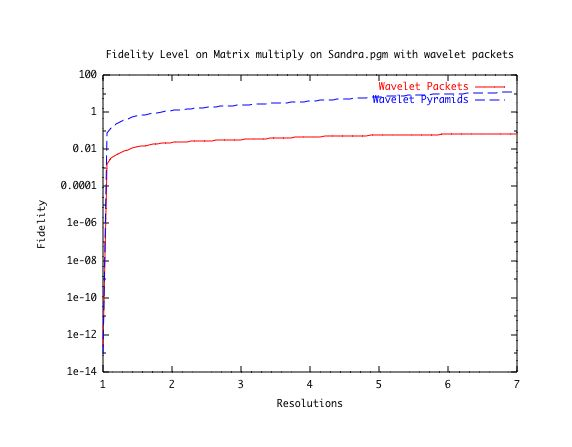
\includegraphics [width=6.5in]{sandrapyrpackresults.jpg}
\caption{This fidelity level graph shows that the wavelet transform packet method as a preconditioner to matrix multiplication is not reliable past the first resolution. The wavelet packet produces marginal results mostly due sections being placed out of order.}
\label{packetresultsstraight}
\end{figure}

\begin{figure}[ht]
\begin{center}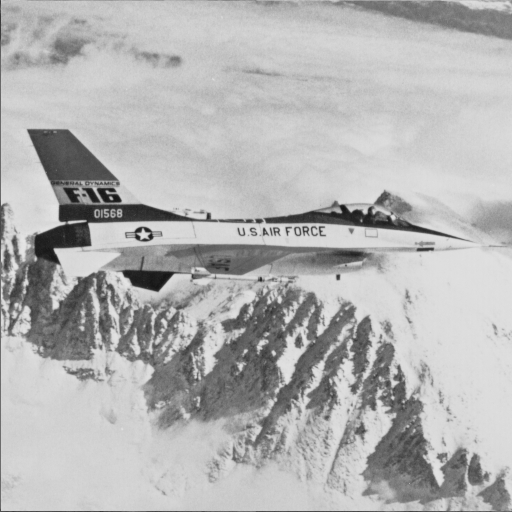
\includegraphics [width=3in]{f16.jpg}\end{center}
\caption{This image is a photo of an F-16 fighter jet.}
\label{imagef16}
\end{figure}
\begin{figure}[ht]
\begin{center}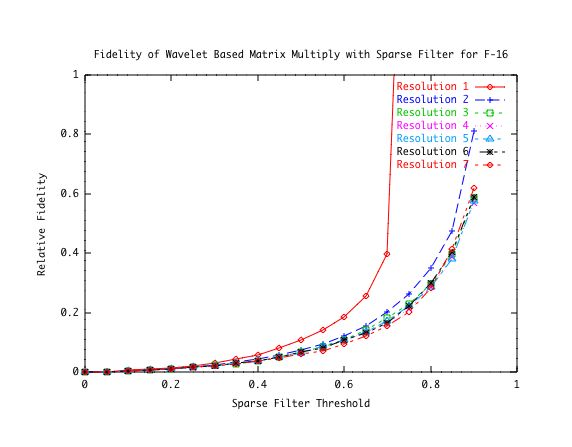
\includegraphics [width=5in]{f16resultsA.jpg}\end{center}
\caption{This fidelity level graph shows that Psi Wavelet Transform (full decomposition) approximation error in matrix multiplication.  This graph in particular was obtained by multiplying the F-16 image by itself with various resolution levels of Wavelet Transforms applied  }
\label{imagef16Fidelity}

\end{figure}

\begin{figure}[ht]
\begin{center}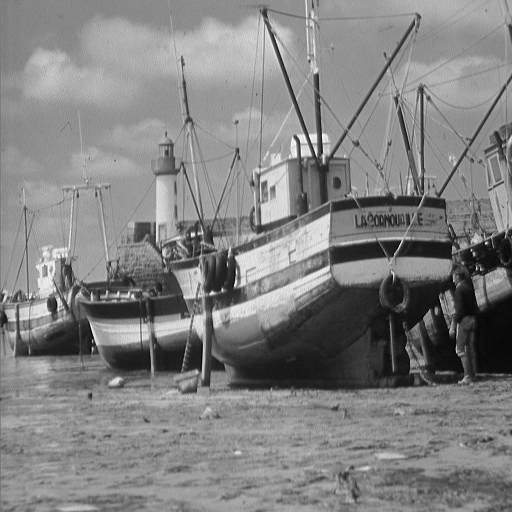
\includegraphics [width=3in]{fishingboat.jpg}\end{center}
\caption{This image is a photo of an Fishing Boat  which is a standard image.}
\label{imagefishingboat}
\end{figure}



\begin{figure}[ht]
\begin{center}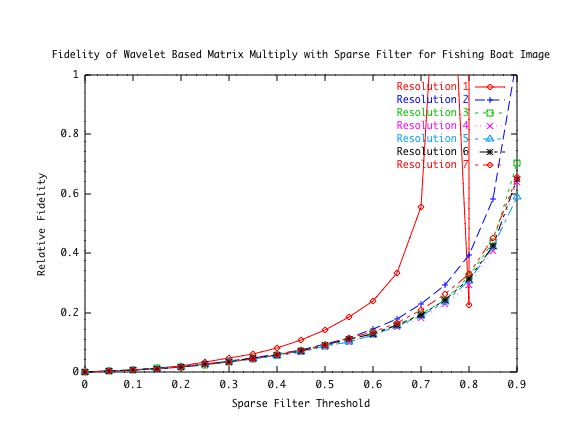
\includegraphics [width=5in]{fishingboatresultA.jpg}\end{center}
\caption{This fidelity level graph shows that Psi Wavelet Transform (full decomposition) approximation error in matrix multiplication.  This graph in particular was obtained by multiplying the Fishing Boat image by itself with various resolution levels of Wavelet Transforms applied.  }
\label{imagefishingboatFidelity}
\end{figure}


\begin{figure}
\begin{center}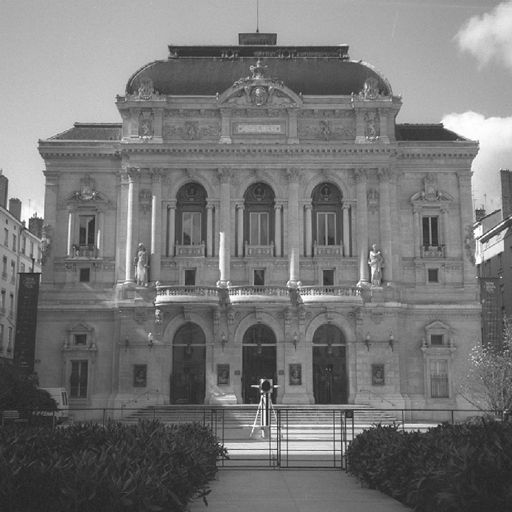
\includegraphics [width=3in] {opera.jpg}\end{center}
\caption {This image is a photo of the Opera House in Lyon \cite{opera}.}
\label{operahouse}
\end{figure}

\begin{figure}[ht]
\begin{center}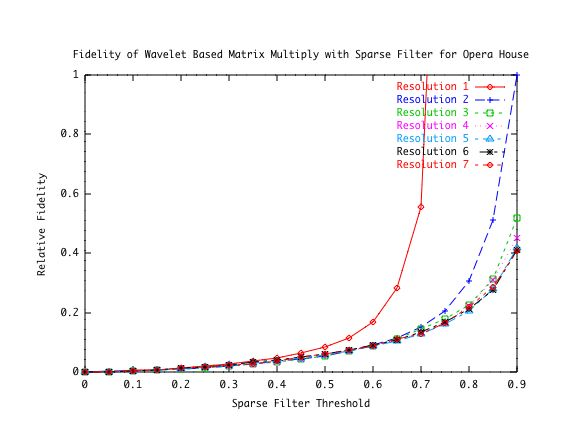
\includegraphics [width=5in]{operaresultsA.jpg}\end{center}
\caption{This fidelity level graph shows that Psi Wavelet Transform (full decomposition) approximation error in matrix multiplication.  This graph in particular was obtained by multiplying the Opera House image by itself with various resolution levels of Wavelet Transforms applied.    }
\label{imageoperaFidelity}
\end{figure}

\begin{figure}[ht]
\begin{center}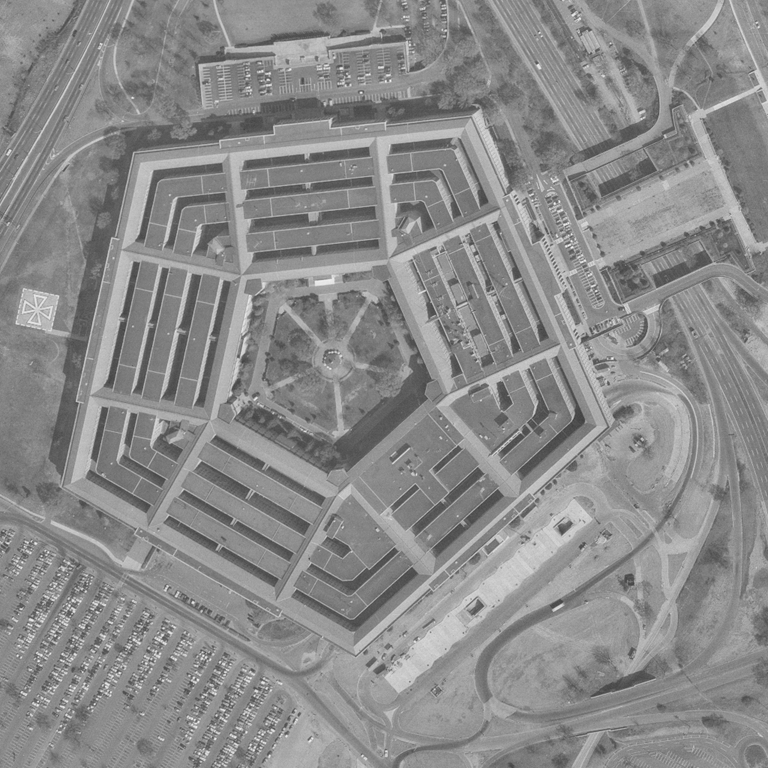
\includegraphics [width=3in]{pentagon.jpg}\end{center}
\caption{This image is an aerial photo of the Pentagon.} % provided Courtesy of the Signal and Image Processing Institute at the University of Southern California.  \cite{pentagon}  This graph in particular was obtained by multiplying the Pentagon image by itself with various resolution levels of Wavelet Transforms applied.  }
\label{imagepentagon}
\end{figure}

\begin{figure}[ht]
\begin{center}\includegraphics [width=5in]{pentagonresultsA.jpg}\end{center}
\caption{This fidelity level graph shows that Psi Wavelet Transform (full decomposition) approximation error in matrix multiplication.  This graph in particular was obtained by multiplying the Pentagon image by itself with various resolution levels of Wavelet Transforms applied. }
\label{imagepentagonFidelity}
\end{figure}

\begin{figure}[ht]
\begin{center}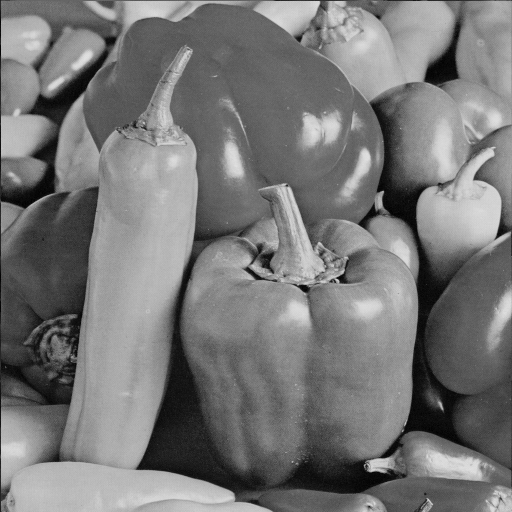
\includegraphics [width=3in]{peppers.jpg}\end{center}
\caption{This image is of peppers was used to populate a sample matrix used to test matrix multiplication.  }
\label{imagePeppers}
\end{figure}

\begin{figure}[ht]
\begin{center}\includegraphics [width=5in]{peppersresultsA.jpg}\end{center}
\caption{This fidelity level graph shows that Psi Wavelet Transform (full decomposition) approximation error in matrix multiplication.  This graph in particular was obtained by multiplying the Peppers image by itself with various resolution levels of Wavelet Transforms applied\cite{peppers}. }
\label{imagepeppersFidelity}
\end{figure}

\begin{figure}[ht]
\begin{center}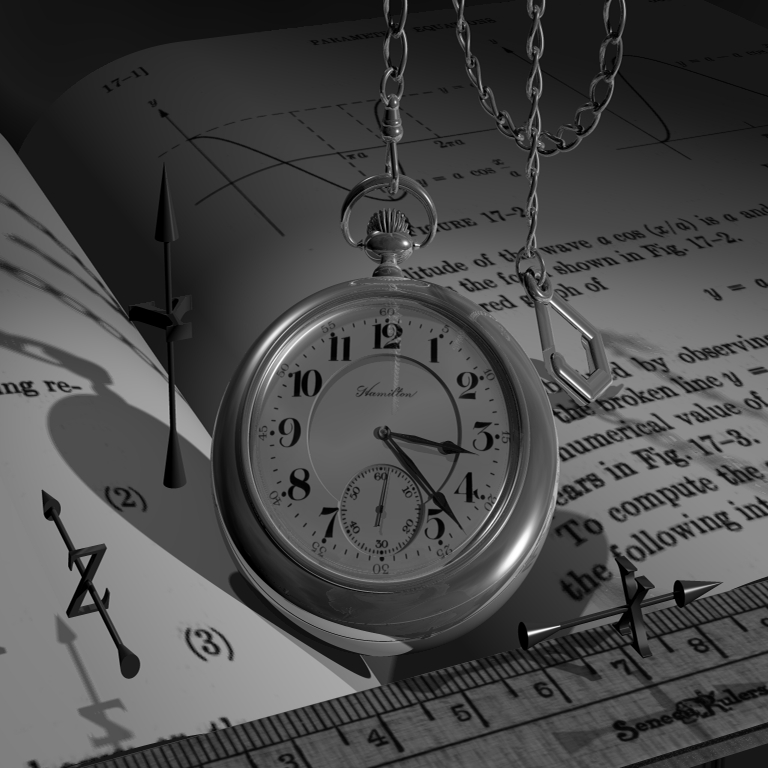
\includegraphics [width=3in]{watch.jpg}\end{center}
\caption{``Pocket Watch on a Gold Chain.'' Copyright image courtesy of Kevin Odhner\cite{watch}.}
\label{imagewatch}
\end{figure}

\begin{figure}[ht]
\begin{center}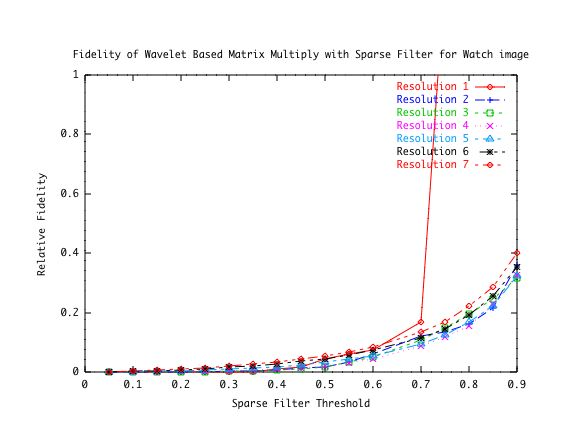
\includegraphics [width=5in]{watchResultsB.jpg}\end{center}
\caption{This fidelity level graph shows that Psi Wavelet Transform (full decomposition) approximation error in matrix multiplication.  This graph in particular was obtained by multiplying the Watch image by itself with various resolution levels of Wavelet Transforms applied \cite{watch}.  }
\label{imagewatchFidelity}
\end{figure}

\begin{figure}[ht]
\begin{center}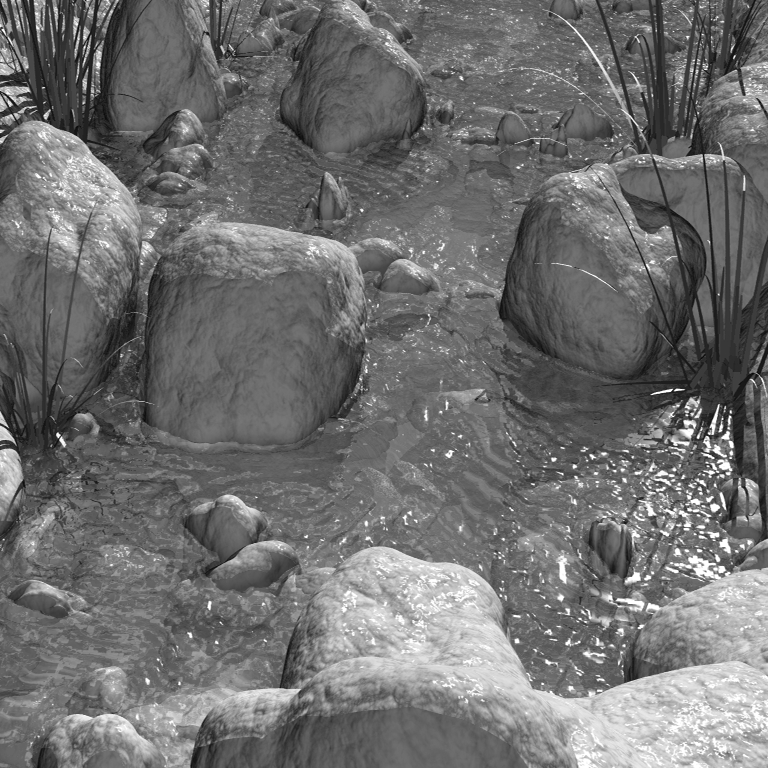
\includegraphics [width=3in]{water.jpg}\end{center}
\caption{This image is an aerial photo of  ``Always running, never the same....'' provided Courtesy of the Jaime Vives Piqueres\cite{water}.}
\label{imagewater}
\end{figure}

\begin{figure}[ht]
\begin{center}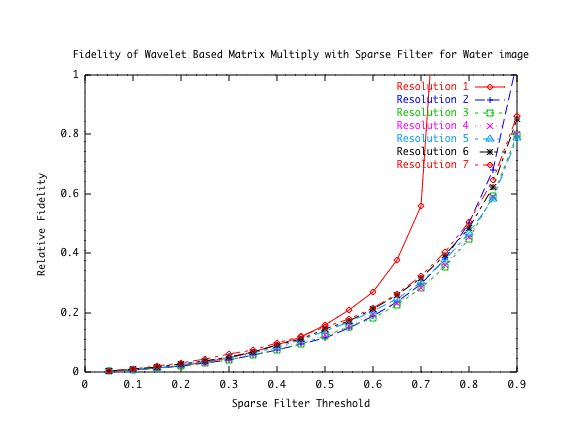
\includegraphics [width=5in]{waterResultsA.jpg}\end{center}
\caption{This fidelity level graph shows that Psi Wavelet Transform (full decomposition) approximation error in matrix multiplication.  This graph in particular was obtained by multiplying the Water image by itself with various resolution levels of Wavelet Transforms applied\cite{water}.}
%\label{imagewaterfallFidelity}
\end{figure}

%{  imagewatch   , imagewater , imagewaterfall}
% {imagef16  ,imagefishingboat  , imageopera,  imagepentagon ,imagepeppers ,imagewatch ,  imagewater  ,imagewaterfall }
% {imagef16Fidelity  ,imagefishingboatFidelity  , imageoperaFidelity,  imagepentagonFidelity ,imagepeppersFidelity ,imagewatchFidelity ,  imagewater  ,imagewaterfallFidelity }

\begin{figure}[ht]
\begin{center}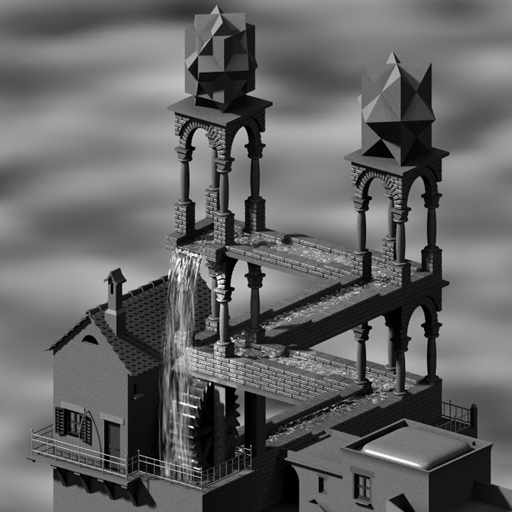
\includegraphics [width=3in]{waterfall.jpg}\end{center}
\caption{Raytraced representation of M.C.Escher's (1898-1972) famous lithography
'Waterfall' (1961), based upon an illusion drawn by
Roger Penrose \cite{waterfall}. }
\label{imagewaterfall}
\end{figure}
\begin{figure}[ht]
\begin{center}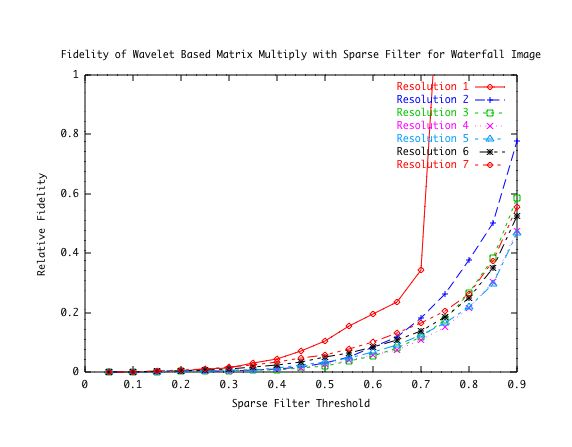
\includegraphics [width=5in]{waterfallResultsA.jpg}\end{center}
\caption{This fidelity level graph shows that Psi Wavelet Transform (full decomposition) approximation error in matrix multiplication.  This graph in particular was obtained by multiplying the Waterfall image by itself with various resolution levels of Wavelet Transforms applied.  \cite{waterfall}  }
\label{imagewaterfallFidelity}
\end{figure}

%\begin{thebibliography}{99}
%\bibitem {waterfall} Sascha Ledinsky \textsl{Waterfall} http://oz.irtc.org/ftp/pub/stills/1998-10-31/waterfa1.txt Internet Raytracing Competition copyright October 31, 1998
%\bibitem {water} Jaime Vives Piqueres \textsl {Always running, never the same...} http://oz.irtc.org/ftp/pub/stills/1998-10-31/running.txt  Internet Raytracing Competition copyright October 31, 1998
%\bibitem {watch} Kevin Odhner \textsl {Pocket Watch on a Gold Chain} 
%\bibitem {opera} fabien a. p. petitcolas {Opera House of Lyon} open domain
%\bibitem {pentagon} Signal and Image Processing Institute at the University of Southern California \textsl{Pentagon} The copyright status of this images in unclear.
%\bibitem {f16}  Signal and Image Processing Institute at the University of Southern California \textsl{F-16}
% The copyright status of this images in unclear.
%\bibitem  {peppers} Signal and Image Processing Institute at the University of Southern California \textsl {Peppers} The copyright status of this images in unclear.
%\bibitem {fishingboat} Signal and Image Processing Institute at the University of Southern California \textsl {Fishing Boat} The copyright status of this images in unclear.

%\end {thebibliography}
% \end{document} 
